\documentclass[a4paper,11pt,twoside,openany]{book}

\usepackage{tipx}
\usepackage[named]{libtex/algo}
\usepackage{algorithm}
\usepackage[noend]{algorithmic}
\usepackage{amssymb}
\setcounter{tocdepth}{3}
\usepackage{graphicx}
\usepackage{amsfonts}
\usepackage{epsfig}
\usepackage{multirow}
\usepackage{amsfonts,amsmath}
\usepackage{srcltx}
\usepackage{multirow}
\usepackage{dsfont}
\usepackage{booktabs}
\usepackage{subfloat}
\usepackage{subcaption}
\usepackage{color}
\usepackage[table]{xcolor}
\usepackage{tabularx}
\usepackage{subfig}
\usepackage{url}
\usepackage{makeidx}
\usepackage{graphicx}
\usepackage{libtex/thesisStyle}


%%%%%%%%%%%%%
\long\def\comment#1{}


\newlength{\figtblfootnotemargin}
\newlength{\figtblfootnotewidth}

\setlength{\figtblfootnotemargin}{15mm}
\setlength{\figtblfootnotewidth}{\textwidth}
\addtolength{\figtblfootnotewidth}{-\figtblfootnotemargin}


%---------------------------------

\newcommand{\db}[1]{
    {\tt #1}
}

%---------------------------------
\newcommand{\outcomment}[1]{
    %\comment{
    \begin{quote}
       {\scriptsize
       {\em OC:} #1
%        #1
       }
    \end{quote}
    %}
}

%---------------------------------

\newcommand{\myheader}[1]{
    \godown
    $\bullet$ {\bf #1} \nn
}

%---------------------------------

\newcommand{\SquareOfSize}[2]{
 \fbox{\hsize #1cm \hbox to #1cm{\vbox{#2}}}
}

\newcommand{\figSquare}[1]{
   \hfill
        \SquareOfSize{13}
            { \vparag \vparag #1 \vparag \vparag }
    \hfill
}

\newcommand{\figSquareLarge}[1]{
   \hfill
        \SquareOfSize{16}
            { \vparag \vparag #1 \parag \vparag }
    \hfill
}

\newcommand{\SQUARE}[1]{
        \SquareOfSize{15}{#1}
}

\newcommand{\SquareSlite}[1]{
        \SquareOfSize{16}{#1}
}


\newcommand{\Syntax}[2]{ ``#1'', where #2 }

\newcommand{\SYNTAX}[2]{
    \SquareOfSize{14}{ \small
        #1 \hfill #2
    }
}

\newcommand{\UpdateProcess}[1]{
    \SquareOfSize{14}{  \bf
        #1
    }
}


\newcommand{\mathdef}[1]
{
    {\small
    \bq {\em Definition.}
        #1
    \eq
    }
}

\newcommand{\pqiCom}[2]{
    \parbox[t]{2cm}{#1} \ \parbox[t]{13.5cm}{ #2}
}

\newcommand{\KEYPOINT}[2]{
\SQUARE{\parbox[t]{3cm}{\small \em  #1} \ \parbox[t]{10cm}{{\bf #2}}}}

%\newcommand{\KEYPOINT}[2]{
%\SQUARE{\small \em  #1: \ \ \parbox[t]{10cm}{{\bf #2}}}}

%___________________________________________________________
\newcommand{\conclusion}[3]{
 \bc
    $ \left.  \begin{array}{r}
                    #1 \\
                    #2
                \end{array}
                    \right\}  \rightarrow #3
            $
 \ec
}
%___________________________________________________________

%-------- Update Operations --------------

\newcommand{\BriefDescription}{$\bullet$
    {\em ������� ���������:} \\}

\newcommand{\CheckedConstraint}
   {$\bullet$ {\em ���������� ������� ����������� :} \\}

\newcommand{\ExecutionAnalysis}[1]{
    $\bullet$ {\em ��������� ��������� :} \\
    \parbox[t]{2cm}{\hspace{2cm}} \ \parbox[t]{12cm}{ {\small #1} }
}

\newcommand{\SemanticAnalysis}[1]{
    $\bullet$ {\em ������������ �������������� ��������� :} \\
    \parbox[t]{2cm}{\hspace{2cm}} \ \parbox[t]{12cm}{ {\small #1} }
}

\newcommand{\namecheck}{ ������� ��������� ���� ������������ }

%--------  ---------------- --------------

\newcommand{\EFupdate}[3]{
    \item  {\scriptsize �����}: #1 {\scriptsize ��������} : $#2$

    \hspace*{1cm} \parbox[t]{12cm}{#3}
}

\newcommand{\visiblecomment}[1]{
  \underline{\centerline{ \bf ������}}\\
     \vspace{0.3cm}
     \bc
      \parbox[t]{14cm}{
            \small \em #1
      } \\
    \ec
  \underline{\centerline{ \bf ����� �������}}
}

\newcommand{\slidefigure}[3]{
% \slidefigure{#1 figure_text}
%             {#2 figure_name}
%             {#3 height_in_mm}

    \begin{figure}[ht]
                    \comment{\rule[0.2in]{\textwidth}{.01in}}
        {\Large \mbox{#1}}
        \centerline{
            \psfig{figure=#2,height=#3}
        }
    \end{figure}
}



\newcommand{\putsinglefigureR}[2]{
% \putsinglefigure{#1 figure_name}
%                 {#2 height_in_mm}

    \begin{figure}[htbp]
        \psfig{figure=#1,height=#2}
    \end{figure}
}

\newcommand{\putsinglefigure}[2]{
% \putsinglefigure{#1 figure_name}
%                 {#2 height_in_mm}

%   \begin{figure}[htbp]            <- not supported in landscape !
        \centerline{
        \psfig{figure=#1,height=#2}
        }
%   \end{figure}
}

\newcommand{\putsfigure}[2]{
        \psfig{figure=#1,height=#2}
}

\newcommand{\putfigure}[5]{
% \putfigure{#1 figure_name}
%           {#2 height_in_mm}
%           {#3 figure_label}
%           {#4 figure_title}
%           {#5 figure_text}

    \begin{figure}[htbp]
        \centerline{ \psfig{figure=#1,height=#2}}
        %\vspace*{-0.3cm} % added 4/5/2001 for EJM conf
        \caption{#4}{\vspace*{0.01cm}  \centerline{ \parbox[t]{13cm}{\footnotesize #5}}}
        \label{#3}
        %\vspace*{-0.6cm} % added 4/5/2001 for EJM conf
    \end{figure}
}



\newcommand{\putfigureVLDB}[5]{
% \putfigure{#1 figure_name}
%           {#2 height_in_mm}
%           {#3 figure_label}
%           {#4 figure_title}
%           {#5 figure_text}

    \begin{figure}[htbp]
        \centerline{ \psfig{figure=#1,height=#2}}
        \vspace*{-0.3cm} % added 4/5/2001 for EJM conf
        \caption{#4}{\vspace*{0.01cm}  \centerline{ \parbox[t]{9cm}{\footnotesize #5}}}
        \label{#3}
        \vspace*{-0.6cm} % added 4/5/2001 for EJM conf
    \end{figure}
}


\newcommand{\putfigureSV}[5]{
% \putfigurSVe{#1 figure_name}  SV = for Springer-Verlag
%           {#2 height_in_mm}
%           {#3 figure_label}
%           {#4 figure_title}
%           {#5 figure_text}

    \begin{figure}[htbp]
        \vspace*{-0.2cm}
        %\vspace*{-0.4cm}
        \centerline{ \psfig{figure=#1,height=#2}}
        \vspace*{-0.3cm}
        \caption{#4}{\vspace*{0.02cm}  \centerline{ \parbox[t]{10cm}{ #5}}}
        \label{#3}
        \vspace*{-0.8cm}
    \end{figure}
}


\newcommand{\putgeneralfigureNEW}[4]{
%           {#1 figure body}
%           {#2 figure_label}
%           {#3 figure_title}
%           {#4 figure_text}
    \begin{figure}[htbp]
        #1
        \vspace*{-0.5cm} % added 4/5/2001 for EJM conf
        \caption{#3}{\vspace*{0.001cm} \centerline{ \parbox[t]{13cm}{\footnotesize #4}}}
        %\caption{#3}{\vspace*{0.1cm} \centerline{ \parbox[t]{\textwidth}{\footnotesize #4}}}
        \label{#2}
        \vspace*{-0.4cm} % added 4/5/2001 for EJM conf
    \end{figure}
}

\newcommand{\putgeneralfigure}[4]{
%           {#1 figure body}
%           {#2 figure_label}
%           {#3 figure_title}
%           {#4 figure_text}

    \begin{figure}[htbp]
        #1
        \vspace*{-0.5cm} % added 4/5/2001 for EJM conf
        \caption{#3}{\vspace*{0.001cm} \centerline{ \parbox[t]{13cm}{\footnotesize #4}}}
        %\caption{#3}{\vspace*{0.1cm} \centerline{ \parbox[t]{\textwidth}{\footnotesize #4}}}
        \label{#2}
        \vspace*{-0.4cm} % added 4/5/2001 for EJM conf
    \end{figure}
}


\newcommand{\putTwoFiguresEngl}[6]{
    \begin{center}
    \begin{figure}
        \begin{minipage}[b]{0.5\textwidth}  %{7cm}
            \centerline{\putsfigure{#1}{#3}}
            \vspace*{3mm} \centerline{(a)}
        \end{minipage}
        \hspace*{0.5cm}
        \begin{minipage}[b]{0.5\textwidth}  %{7cm}
            \centerline{\putsfigure{#2}{#3}}
            \vspace*{3mm} \centerline{(b)}
        \end{minipage}
        \caption{#5}{\vspace*{0.1cm}
            \centerline{ \parbox[t]{13cm}{\footnotesize #6}}}
        \label{#4}
        \vspace*{-5mm} % added 15/9/2004
    \end{figure}
    \end{center}
}



\newcommand{\putTwoFiguresEnglSquare}[6]{
    %\begin{center}
    \begin{figure}
        \begin{minipage}[b]{85mm}
            \centerline{\fbox{\putsfigure{#1}{#3}}}
            \vspace*{3mm} \centerline{(a)}
        \end{minipage}
        \begin{minipage}[b]{85mm}
            \centerline{\fbox{\putsfigure{#2}{#3}}}
            \vspace*{3mm} \centerline{(b)}
        \end{minipage}
        \vspace*{-0.3cm}
        \caption{#5}{\vspace*{0.1cm}
            \centerline{ \parbox[t]{13cm}{\footnotesize #6}}}
        \label{#4}
        \vspace*{-8mm} % added 15/9/2004
    \end{figure}
    %\end{center}
}

\newcommand{\putFourFiguresEnglSquare}[8]{
    %\begin{center}
    \begin{figure}
        \begin{minipage}[b]{40mm}
            \centerline{\fbox{\putsfigure{#1}{#5}}}
            \vspace*{3mm} \centerline{(a)}
        \end{minipage}
        \begin{minipage}[b]{40mm}
            \centerline{\fbox{\putsfigure{#2}{#5}}}
            \vspace*{3mm} \centerline{(b)}
        \end{minipage}
        \begin{minipage}[b]{40mm}
            \centerline{\fbox{\putsfigure{#3}{#5}}}
            \vspace*{3mm} \centerline{(c)}
        \end{minipage}

        \begin{minipage}[b]{40mm}
            \centerline{\fbox{\putsfigure{#4}{#5}}}
            \vspace*{3mm} \centerline{(d)}
        \end{minipage}
        \caption{#7}{\vspace*{0.1cm}
            \centerline{ \parbox[t]{13cm}{\footnotesize #8}}}
        \label{#6}
        \vspace*{-1mm} % added 15/9/2004
        %\vspace*{-8mm} % added 15/9/2004
    \end{figure}
    %\end{center}
}

\newcommand{\putFigureAndText}[6]{
    \begin{figure}
        \begin{minipage}[b]{7cm}
            \centerline{\putsfigure{#1}{#2}}
            \vspace*{1mm} \centerline{(a)}
        \end{minipage}
        \begin{minipage}[b]{7cm}
            \bc
                #6
            \ec
            \vspace*{1mm} \centerline{(b)}
        \end{minipage}
        \caption{#4}{\vspace*{-2mm}
            \centerline{ \parbox[t]{13cm}{\footnotesize #5}}}
        \label{#3}
         %\vspace*{-10mm} % added 25/10/2001 for WISE conf
         %\vspace*{-5mm} % added 25/10/2001 for SETNT conf
    \end{figure}
}

% lala
\newcommand{\putFigureAndTextSV}[6]{
    \begin{figure}
        \vspace*{-0.4cm}   % SV
        \begin{minipage}[b]{6cm}
            \centerline{\putsfigure{#1}{#2}}
            \vspace*{1mm} \centerline{(a)}
        \end{minipage}
        \begin{minipage}[b]{6cm}
            \bc
                #6
            \ec
            \vspace*{1mm} \centerline{(b)}
        \end{minipage}
        \caption{#4}{\vspace*{-2mm}
            \centerline{ \parbox[t]{13cm}{\footnotesize #5}}}
        \label{#3}
        \vspace*{-8mm} %
    \end{figure}
}

\newcommand{\putFigureAndTextVLDB}[6]{
    \begin{figure}[h]
        \begin{minipage}[b]{7cm}
            \centerline{\putsfigure{#1}{#2}}
            \vspace*{1mm} \centerline{(a)}
        \end{minipage}
        \begin{minipage}[b]{7cm}
            \bc
                #6
            \ec
            \vspace*{1mm} \centerline{(b)}
        \end{minipage}
        \caption{#4}{%\vspace*{-2mm}
            \centerline{ \parbox[t]{85mm}{\footnotesize #5}}}
        \label{#3}
         %\vspace*{-10mm} % added 25/10/2001 for WISE conf
         %\vspace*{-5mm} % added 25/10/2001 for SETNT conf
    \end{figure}
}



\newcommand{\putTwoFigures}[6]{
    %\begin{center}
    \begin{figure}
        \begin{minipage}[b]{7cm}
            \centerline{\putsfigure{#1}{#3}}
            \vspace*{3mm} \centerline{(�)}
        \end{minipage}
        \begin{minipage}[b]{7cm}
            \centerline{\putsfigure{#2}{#3}}
            \vspace*{3mm} \centerline{(�)}
        \end{minipage}
        \caption{#5}{\vspace*{0.1cm}
            \centerline{ \parbox[t]{13cm}{\footnotesize #6}}}
        \label{#4}
    \end{figure}
    %\end{center}
}


\newcommand{\putTwoSliteFiguresB}[3]{
    \parbox[b]{7cm}{
            \centerline{\putsfigure{#1}{#3}}
    } \
    \parbox[b]{7cm}{
            \centerline{\putsfigure{#2}{#3}}
    }
}

\newcommand{\putTwoSliteFigures}[3]{
    \begin{figure}[h]
        \begin{minipage}[b]{7cm}
            \centerline{\putsfigure{#1}{#3}}
            %\vspace*{3mm} \centerline{(�)}
        \end{minipage}
        \begin{minipage}[b]{7cm}
            \centerline{\putsfigure{#2}{#3}}
            %\vspace*{3mm} \centerline{(�)}
        \end{minipage}
    \end{figure}
}



\newcommand{\putfigureSquare}[5]{
% \putfigure{#1 figure_name}
%           {#2 height_in_mm}
%           {#3 figure_label}
%           {#4 figure_title}
%           {#5 figure_text}

    \begin{figure}[htbp]
        \centerline{ \fbox{\psfig{figure=#1,height=#2}}}
        %\vspace*{-0.3cm} % added 4/5/2001 for EJM conf
        \vspace*{-0.3cm}
        \caption{#4}{\vspace*{0.01cm}  \centerline{ \parbox[t]{13cm}{\footnotesize #5}}}
        \label{#3}
        %\vspace*{-0.6cm} % added 4/5/2001 for EJM conf
        \vspace*{-0.5cm}
    \end{figure}
}



\newcommand{\puttable}[4]{
% \puttable {#1 table_label}
%           {#2 table_title}
%           {#3 table_text}
%           {#4 table_body}
    \begin{table}[htbp]
        \begin{center}
            #4
            \caption{#2}{\vspace*{0.1cm} \centerline{ \parbox[t]{13cm}{\footnotesize #3}}}
            \label{#1}
        \end{center}
        \vspace*{-0.8cm} % added 25/10/2001 for WISE conf
    \end{table}
}

\newcommand{\putwidetable}[4]{
% \puttable {#1 table_label}
%           {#2 table_title}
%           {#3 table_text}
%           {#4 table_body}
    \begin{table}[htbp]
        %\begin{center}
            \hspace*{5mm}
            #4
            \caption{#2}{\vspace*{0.1cm} \centerline{ \parbox[t]{16cm}{\footnotesize #3}}}
            \label{#1}
        %\end{center}
        %\vspace*{-0.8cm} % added 25/10/2001 for WISE conf
    \end{table}
}

\newcommand{\puttableSV}[4]{  % caption on top
% \puttableSV{#1 table_label}   SV = for Springer-Verlag format
%           {#2 table_title}
%           {#3 table_text}
%           {#4 table_body}
    \begin{table}[htbp]
        \begin{center}
            \vspace*{-3mm} % 8-3-04
            \caption{#2}{\vspace*{-3mm} \centerline{ \parbox[t]{10cm}{ #3}}}
            \vspace*{-3mm} % 7-11-05
            \label{#1}
            #4
        \end{center}
    \end{table}
    \vspace*{-2mm} % 8-3-04
}

\newcommand{\puttableSVold}[4]{  //old version: caption at bottom
% \puttableSV{#1 table_label}   SV = for Springer-Verlag format
%           {#2 table_title}
%           {#3 table_text}
%           {#4 table_body}
    \begin{table}[htbp]
        \begin{center}
            #4
            \caption{#2}{\vspace*{0.01cm} \centerline{ \parbox[t]{10cm}{ #3}}}
            \label{#1}
        \end{center}
    \end{table}
}

\newcommand{\puttableSIGMOD}[4]{  % caption on top
% \puttableSV{#1 table_label}   SV = for Springer-Verlag format
%           {#2 table_title}
%           {#3 table_text}
%           {#4 table_body}
    \begin{table}[htbp]
        \begin{center}
            %\vspace*{-4mm} % 8-3-04
            \caption{#2}{\centerline{ \parbox[t]{13cm}{ #3}}}
            %\vspace*{-4mm} % 8-3-04
            \label{#1}
            #4
        \end{center}
    \end{table}
    %\vspace*{-5mm} % 8-3-04
}

\newcommand{\putFourTables}[7]{
% \puttable {#1 table_label}
%           {#2 table_title}
%           {#3 table_text}
%           {#4 table_body1}
%           {#5 table_body2}
%           {#6 table_body3}
%           {#7 table_body4}
    \begin{table}[htbp]
        \begin{center}
            #4 #5 #6 #7
            \caption{#2}{\vspace*{0.1cm} \centerline{ \parbox[t]{13cm}{\footnotesize #3}}}
            \label{#1}
        \end{center}
    \end{table}
}





\newcommand{\putalgorithm}[2]{
% \putalgorithm {#1 alg_label}^M
%               {#2 alg_body}^M
    \begin{figure}[htbp]
        %\underline{\hspace*{16cm}}
        {\bf Algorithm} \label{#1}.

        #2

        %\underline{\hspace*{16cm}}
    \end{figure}
}



% Changes page margins :
%   eg \begin{changemargin}{-1cm}{-1cm}  ( widens page )
%   eg \begin{changemargin}{2cm}{2cm}    ( narrows page )
%
\newenvironment{changemargin}[2]{\begin{list}{}{
         \setlength{\topsep}{0pt}
          \setlength{\leftmargin}{0pt}
         \setlength{\rightmargin}{0pt}
         \setlength{\listparindent}{\parindent}
         \setlength{\itemindent}{\parindent}
         \setlength{\parsep}{0pt plus 1pt}
         \addtolength{\leftmargin}{#1}\addtolength{\rightmargin}{#2}
         }\item }{\end{list}
}

\newsavebox{\wholeWidthLine}
\sbox{\wholeWidthLine} {\rule[0.1in]{\textwidth}{.01in}}

\newcommand{\Figure}[5] {
%           {#1 figure_body}
%           {#2 figure_label}
%           {#3 figure_title}
%           {#4 figure_text}
%           {#5 figure_placement}
    \begin{figure}[#5]
        %\usebox{\wholeWidthLine}
        \vspace*{2mm}
        #1
        \caption{#3}{\
            \cl{\parbox[t]{\figtblfootnotewidth}{\footnotesize #4}}}
        \label{#2}
        \vspace*{2mm}
        %\usebox{\wholeWidthLine}
    \end{figure}
}


\newcommand{\putAndPlaceGeneralFigure}[5]{
%           {#1 figure body}
%           {#2 figure_label}
%           {#3 figure_title}
%           {#4 figure_text}
%           {#5 figure_placement}
    \begin{figure}[#5]
        %\usebox{\wholeWidthLine}
        \bc
            #1
        \ec
        \caption{#3}{\
            \centerline{\parbox[t]{\figtblfootnotewidth}{\footnotesize #4}}}
        \label{#2}
        %\usebox{\wholeWidthLine}
    \end{figure}
}


\newcommand{\abstrOfeq}[0]{
     \sqsubseteq
}
\newcommand{\abstrOf}[0]{
     \sqsubset
}

%\newcommand{\notisA}[0]{
     %isA \hspace*{-0.6cm} \not  \hspace*{0.6cm}
%}


\newcommand{\mysignature}{
    \parbox[t]{7cm}{
        \begin{center}
            {\normalsize ������� �. ���������} \\
            {\small MSc Computer Science} \\
            {\scriptsize ���: 093 47 13 11, (081) 256 561 }
        \end{center}
    }
}


% Frequently Used commands

\newcommand{\bq}{\begin{quote}}
\newcommand{\eq}{\end{quote}}
\newcommand{\be}{\begin{enumerate}}
\newcommand{\ee}{\end{enumerate}}
\newcommand{\bi}{\begin{itemize}}
\newcommand{\ei}{\end{itemize}}
\newcommand{\bie}{\begin{itemize}\begin{enumerate}}
\newcommand{\eie}{\end{enumerate}\end{itemize}}
\newcommand{\ba}{\begin{array}}
\newcommand{\ea}{\end{array}}
\newcommand{\btbl}{\begin{tabular}}
\newcommand{\etbl}{\end{tabular}}
\newcommand{\bequ}{\begin{displaymath}}
\newcommand{\eequ}{\end{displaymath}}
\newcommand{\bequa}{\begin{eqnarray*}}
\newcommand{\eequa}{\end{eqnarray*}}
\newcommand{\bc}{\begin{center}}
\newcommand{\ec}{\end{center}}
\newcommand{\btab}{\begin{tabbing}}
\newcommand{\etab}{\end{tabbing}}
\newcommand{\cl}{\centerline}

\newcommand{\mysection}[1]{
    \centerline{\LARGE \bf #1}
    \godown
}

\newcommand{\goright}{\hspace*{0.5cm}}
\newcommand{\goRight}{\goright \goright}
\newcommand{\goRIGHT}{\goRight \goRight}

\newcommand{\bul}{ $\bullet$ }
\newcommand{\goup}{ \vspace*{-0.5cm}}
\newcommand{\goUp}{ \goup \goup}
%\newcommand{\goUP}{ \vspace*{-0.5cm}}


\newcommand{\vparag}{ \vskip 5mm}
\newcommand{\godown}{ \vspace*{0.3cm}}
\newcommand{\goDown}{ \godown \godown}
\newcommand{\goDOWN}{ \goDown \goDown }

% set operator : not in
\newcommand{\noin}{\in \hspace{-0.33cm} / \hspace{0.3cm} }

%=========== MATH SYMBOLS ==============

\newcommand{\FALL}{\;\forall \;}
\newcommand{\mybox}[1]{\mbox{\letterspace #1 \letterspace }}
\newcommand{\card}[1]{
        \letterspace\mid
         #1
        \mid\letterspace
}


%=========== MDE WRITING ==============

% mpr : prints its argument in math mode
%       It can also be called from non math mode
\def\mpr#1{\ifmmode #1 \else #1 \fi}

\newcommand{\TB}        {\mpr{TB}}

%\newcommand{\R}         {\mpr{R}}
\newcommand{\RIN}       {\mpr{R^{in}}}
\newcommand{\RINALL}    {\mpr{R^{in}_{impl}}}
\newcommand{\RINB}      {\mpr{R^{in}_{sys}}}
\newcommand{\RINU}      {\mpr{R^{in}_{u}}}
\newcommand{\RINUtonos} {\mpr{R^{in'}_{u}}}
\newcommand{\RISA}      {\mpr{R^{isA}}}
\newcommand{\RISATR}    {\mpr{R^{isA}_{tr}}}
\newcommand{\RISAB}     {\mpr{R^{isA}_{sys}}}
\newcommand{\RISAU}     {\mpr{R^{isA}_{u}}}
\newcommand{\RISAUtonos}{\mpr{R^{isA'}_{u}}}
\newcommand{\RFROM}     {\mpr{R^{from}}}
\newcommand{\RTO}       {\mpr{R^{to}}}

%\newcommand{\TO}        {\mpr{O}}
\newcommand{\TOB}       {\mpr{O_{sys}}}
\newcommand{\TOU}       {\mpr{O_{u}}}
\newcommand{\PV}        {\mpr{PV}}
\newcommand{\Integer}   {\mpr{Integer}}
\newcommand{\Real}      {\mpr{Real}}
\newcommand{\String}    {\mpr{String}}
\newcommand{\Nat}       {\mpr{N}}
\newcommand{\LN}    {\mpr{L}}
\newcommand{\LF}    {\mpr{{\cal L}}}

\newcommand{\TI}        {\mpr{I}}
\newcommand{\TIU}       {\mpr{I_{u}}}
\newcommand{\TA}        {\mpr{A}}
\newcommand{\TC}        {\mpr{C}}
\newcommand{\TIC}       {\mpr{I_{c}}}
\newcommand{\TAC}       {\mpr{A_{c}}}

\newcommand{\type}      {\mpr{type}}
\newcommand{\level}     {\mpr{level}}
\newcommand{\typeb}     {\mpr{type_{sys}}}
\newcommand{\levelb}    {\mpr{level_{sys}}}

\newcommand{\SemT}      {\mpr{SemanticType}}
\newcommand{\SynT}      {\mpr{SyntacticType}}

\newcommand{\semT}      {\mpr{semType}}
\newcommand{\synT}      {\mpr{synType}}
\newcommand{\semTb}     {\mpr{semType_{sys}}}
\newcommand{\synTb}     {\mpr{synType_{sys}}}

\newcommand{\sem}       {\mpr{sem}}
\newcommand{\syn}       {\mpr{syn}}

\newcommand{\PBT}       {\mpr{PBT}}
\newcommand{\TP}        {\mpr{TP}}


%-- TELOS QUERIES

% writting TELOS statements
\newcommand{\telos}{Telos\letterspace}
\newcommand{\clio}{
    % $\cal{K}${\em �}$\cal{EI}${\em �} \letterspace
    {\em �����}
}
\newcommand{\tellretell}{TELL/RETELL\letterspace}
\newcommand{\export}{{\em Export} \letterspace}

\newcommand{\letterspace}{\hspace*{1mm}}

\newcommand{\ison}{\;=\;}
\newcommand{\isA}{\mbox{\bf isA} \letterspace}
\newcommand{\instOf}{\mbox{\bf instOf}}

\newcommand{\Tell}{{\bf TELL Individual} \letterspace}
\newcommand{\Retell}{{\bf RETELL Individual} \letterspace}
\newcommand{\End}{{\bf end} \letterspace}
\newcommand{\inT}{{\bf in} \letterspace}
\newcommand{\scl}{{\bf S\_Class} \letterspace}
\newcommand{\tok}{{\bf Token} \letterspace}

\newcommand{\printPQI}[1]{ \mbox{\bf #1} \letterspace }

\newcommand{\sysclass}{ \printPQI{sysclass}}
\newcommand{\scn}{      \printPQI{scn}}
\newcommand{\gfv}{      \printPQI{gfv}}
\newcommand{\gtv}{      \printPQI{gtv}}
\newcommand{\glf}{      \printPQI{glf}}
\newcommand{\gilf}{     \printPQI{gilf}}
\newcommand{\gilt}{     \printPQI{gilt}}
\newcommand{\glt}{      \printPQI{glt}}
\newcommand{\glfc}{     \printPQI{glfc}}
\newcommand{\gfnc}{     \printPQI{gfnc}}
\newcommand{\gtnc}{     \printPQI{gtnc}}
\newcommand{\gasb}{     \printPQI{gasb}}
\newcommand{\gsb}{      \printPQI{gsb}}
\newcommand{\gasc}{     \printPQI{gasc}}
\newcommand{\gc}{       \printPQI{gc}}
\newcommand{\gac}{      \printPQI{gac}}
\newcommand{\gai}{      \printPQI{gai}}
\newcommand{\gi}{       \printPQI{gi}}
\newcommand{\gsc}{      \printPQI{gsc}}
\newcommand{\gSc}{      \printPQI{gSc}}
\newcommand{\gaSc}{     \printPQI{gaSc}}
\newcommand{\gSi}{      \printPQI{gSi}}
\newcommand{\attrs}{    \printPQI{attrs}}
\newcommand{\focus}     {{\em s \letterspace}}

%---------- CHAPTER 4 -------------------
\newcommand{\BPE}[1]{ \mbox{\bf #1 \letterspace} }

\newcommand{\CreateNode}        {\BPE{CreateIndividual}}
\newcommand{\DeleteNode}        {\BPE{DeleteIndividual}}
\newcommand{\CreateAttribute}   {\BPE{CreateAttribute}}
\newcommand{\DeleteAttribute}   {\BPE{DeleteAttribute}}
\newcommand{\AddInstance}       {\BPE{AddInstance}}
\newcommand{\DeleteInstance}    {\BPE{DeleteInstance}}
\newcommand{\Rename}            {\BPE{Rename}}
\newcommand{\AddSubClass}       {\BPE{AddSubClass}}
\newcommand{\DelSubClass}       {\BPE{DeleteSubClass}}
\newcommand{\makecopy}          {\BPE{MakeCopy}}

%---tmpmaybe
\newcommand{\CreateNodeSet}     {{\em CreateNodeSet}}
\newcommand{\DeleteNodeSet}     {{\em DeleteNodeSet}}
\newcommand{\CreateAttributeSet}{{\em CreateAttributeSet}}
\newcommand{\DeleteAttributeSet}{{\em DeleteAttributeSet}}
\newcommand{\AddInstanceSet}    {{\em AddInstanceSet}}
\newcommand{\DeleteInstanceSet} {{\em DeleteInstanceSet}}
\newcommand{\RenameSet}         {{\em RenameSet}}
\newcommand{\AddSubClassSet}    {{\em AddSubClassSet}}
\newcommand{\DelSubClassSet}    {{\em DelSubClassSet}}

%---------- CHAPTER 5 -------------------
\newcommand{\EFID}[1]{ \mbox{\em \scriptsize #1 } }

\newcommand{\obj}{ \letterspace
                    \mbox{\em o}\letterspace
}
\newcommand{\aobj}{ \mbox{\em a}\letterspace}
\newcommand{\bobj}{ \mbox{\em b}\letterspace}
\newcommand{\fobj}{ \mbox{\em from}\letterspace}
\newcommand{\tobj}{ \mbox{\em to}\letterspace}
\newcommand{\sobj}{ \mbox{\em s}\letterspace}
\newcommand{\cobj}{ \mbox{\em c}\letterspace}
\newcommand{\iobj}{ \mbox{\em i}\letterspace}
\newcommand{\ObjectSet}{ \mybox{\em ObjectSet}}
\newcommand{\SysClass}{ \mbox{\em SysClass}\letterspace}

\newcommand{\CREATENODE}    {\EFID{CREATE\_INDIVIDUAL}}
\newcommand{\DELETENODE}    {\EFID{DELETE\_INDIVIDUAL}}
\newcommand{\RENAMENODE}    {\EFID{RENAME\_INDIVIDUAL}}
\newcommand{\CHANGECLASSES} {\EFID{CHANGE\_CLASSES}}
\newcommand{\CHANGESUPERCLASSES}{\EFID{CHANGE\_SUPERCLASSES}}
\newcommand{\CHANGEATTRIBUTES}  {\EFID{CHANGE\_ATTRIBUTES}}
\newcommand{\nullset}   {-\hspace*{-0.1cm}-}
%%\newcommand{\emptyset}    {0\hspace*{-0.1cm}\/}
%\newcommand{\concat}   {\letterspace\#\letterspace}
\newcommand{\concat}    {\letterspace\circ\letterspace}

\newcommand{\DC}{
        \letterspace {\bf DC}\letterspace
}
\newcommand{\DO}{
        \letterspace {\bf DO}\letterspace
}
\newcommand{\RC}{${\cal R}\;$}
\newcommand{\calA}{${\cal A}\;$}
\newcommand{\calB}{${\cal B}\;$}
\newcommand{\calE}{${\cal E}\;$}

%---------- CHAPTER 6 -------------------

\newcommand{\mmName}{ ���� }

\newcommand{\sneg}   { \mbox{\={$\! \! \! s$}} }

\newcommand{\Users}      {Users}
\newcommand{\SystemUsers}{SystemUsers}
\newcommand{\UserTypes}  {UserTypes}

\newcommand{\Ustx}       {U_{stx}}
\newcommand{\Usem}       {U_{sem}}
\newcommand{\Tasks}      {Tasks}
\newcommand{\tsem}      {t_{sem}}
\newcommand{\apon}          {applyon}
\newcommand{\aponsem}       {applyon_{sem}}
\newcommand{\aponsemt}      {applyon^{t}_{sem}}

\newcommand{\SetIds}    {ID}
\newcommand{\tids}      {S_{id}}
\newcommand{\tidsR}     {S^{-1}_{id}}

\newcommand{\pids}      {P^{expl}_{id}}
\newcommand{\nids}      {N^{expl}_{id}}
\newcommand{\pimids}    {P^{impl}_{id}}
\newcommand{\nimids}    {N^{impl}_{id}}

\newcommand{\ti}        {S_{i}}
\newcommand{\tiR}       {S^{-1}_{i}}
\newcommand{\tj}        {S_{j}}

\newcommand{\cro}       {CrObj}
\newcommand{\delo}      {DelObj}
\newcommand{\ren}       {REN}
\newcommand{\del}       {DEL}
\newcommand{\addaf}     {AddAF}
\newcommand{\addat}     {AddAT}
\newcommand{\delaf}     {DelAF}
\newcommand{\delat}     {DelAT}
\newcommand{\addin}     {AddIn}
\newcommand{\delin}     {DelIn}
\newcommand{\addsub}    {AddSub}
\newcommand{\delsub}    {DelSub}
\newcommand{\addsup}    {AddSup}
\newcommand{\delsup}    {DelSup}
\newcommand{\addclass}  {AddClass}
\newcommand{\delclass}  {DelClass}

\newcommand{\tcro}      {S_{\cro}}
\newcommand{\tcroR}     {S^-1_{\cro}}
\newcommand{\tdelo}     {S_{\delo}}
\newcommand{\tdeloR}    {S^-1_{\delo}}
\newcommand{\tren}      {S_{\ren}}
\newcommand{\tdel}      {S_{\del}}
\newcommand{\taddaf}    {S_{\addaf}}
\newcommand{\tdelaf}    {S_{\delaf}}
\newcommand{\taddat}    {S_{\addat}}
\newcommand{\tdelat}    {S_{\delat}}
\newcommand{\taddin}    {S_{\addin}}
\newcommand{\tdelin}    {S_{\delin}}
\newcommand{\taddsub}   {S_{\addsub}}
\newcommand{\tdelsub}   {S_{\delsub}}


\newcommand{\negS}      {{\scriptsize NEG}}
\newcommand{\posS}      {{\scriptsize POS}}
\newcommand{\noneS}     {{\scriptsize NONE}}

\newcommand{\QT}    {{\cal QT}}

\newcommand{\symboleq}  {\stackrel{����}{=}}

\newcommand{\qlevel}        {level}
\newcommand{\qlevelsub}     {levelsub}
\newcommand{\qsubs}         {subs}
\newcommand{\qgai}      {gai}
\newcommand{\qglf}      {glf}
\newcommand{\qglfgasb}  {glfgasb}

\newcommand{\Rules}     {{\cal R}}
\newcommand{\ARules}    {{\cal A}}
\newcommand{\Preds}     {{\cal PR}}
\newcommand{\PredTypes} {{\cal PRT}}
\newcommand{\PredSys}   {{\cal PR}_{sys}}
\newcommand{\PredIN}    {{\cal PR}_{in}}
\newcommand{\PredAIN}   {{\cal PR}_{ain}}
\newcommand{\PredASUB}  {{\cal PR}_{asub}}
\newcommand{\PredL}     {{\cal PR}_{links}}
\newcommand{\PredASUBL} {{\cal PR}_{sublinks}}

%\newcommand{\TRUE}  {{\small \mbox{TRUE}}}

%---------- CHAPTER 6  <OLDVERSION> ---------
%----- S Q L ---------

    \newcommand{\sql}[1]{{\bf #1}}

    \newcommand{\SELVIEW}[1]{
        \sql{SELECTION VIEW} {\em #1}
    }
    \newcommand{\SELVIEWslite}[1]{
        \sql{SELECTION VIEW} #1
    }

    \newcommand{\FROM}[2]{
        \hspace*{1cm} \sql{FROM} {\em #1} \sql{IN} {\em #2}
    }
    \newcommand{\FROMslite}[2]{
        \hspace*{1cm} \sql{FROM} #1 \sql{IN} #2
    }

    \newcommand{\WHERE}[1]{
        \hspace*{1cm} \sql{WHERE} {\em #1}
    }
    \newcommand{\WHEREslite}[1]{
        \hspace*{1cm} \sql{WHERE} #1
    }

%---------------

\newcommand{\oos}[1]{ \mbox{\bf #1} }

%--- UIDS
\newcommand{\printUID}[1]{ \mbox{\em #1} }


\newcommand{\SCuid}[0]      { \printUID{Schema} }

\newcommand{\INuid}[0]      { \printUID{IN} }
\newcommand{\IDuid}[0]      { \printUID{ID} }
\newcommand{\ISAuid}[0]     { \printUID{ISA} }
\newcommand{\NAMEuid}[0]    { \printUID{NAME} }
\newcommand{\ATTRSuid}[0]   { \printUID{ATTR} }
\newcommand{\INSTATTRSuid}[0]{\printUID{INST\_ATTRS} }


%---- Update Sets

\newcommand{\UT}{ UpdateTypes}
\newcommand{\US}{ UpdateState}
\newcommand{\UID}{ UpdateIDs}

\newcommand{\where}[0]{
    \mbox{ \letterspace ����  \letterspace}
}
\newcommand{\an}[0]{
    \mbox{ \letterspace ��  \letterspace}
}
\newcommand{\then}[0]{
    \mbox{ \letterspace ����  \letterspace}
}
\newcommand{\kai}[0]{
    \mbox{ \letterspace ���  \letterspace}
}
\newcommand{\whereT}[0]{
    \mbox{t $\in$ \UT}
}
\newcommand{\Change}{ \mbox{ Changable} }
\newcommand{\Invariant}{ \mbox{ Invariant} }

\newcommand{\Inv}[1]{ \mbox{ Inv[#1]} }
\newcommand{\Ch}[1]{ \mbox{ Ch[#1]} }

\newcommand{\Invv}[2]{ \mbox{ Inv[#1][#2]} }
\newcommand{\Chh}[2]{ \mbox{ Ch[#1][#2]} }

\newcommand{\InvExpl}[1]{ \Invv{Expl}{#1} }
\newcommand{\ChExpl}[1]{ \Chh{Expl}{#1} }

\newcommand{\InvSub}[1]{ \Invv{onSubs}{#1} }
\newcommand{\ChSub}[1]{ \Chh{onSubs}{#1} }

\newcommand{\InvAttr}[1]{ \Invv{onAttrsFrom}{#1} }
\newcommand{\ChAttr}[1]{ \Chh{onAttrsFrom}{#1} }

\newcommand{\InvAttrSub}[1]{ \Invv{onAttrsSubFrom}{#1} }
\newcommand{\ChAttrSub}[1]{ \Chh{onAttrsSubFrom}{#1} }

\newcommand{\Existencial}{\mbox{Existencial}}




\newtheorem{telos_rule}{�����������}
\newtheorem{my_rule}{�������}

\newcommand{\subjectCondition} {{\em ������� ��� \obj :}}
\newcommand{\argumentCondition}{{\em ������� ��� �������� :} }

\newcommand{\argset}[1]{{\em ������ ������� #1 :} }

%\newcommand{\DPATTRNAME}{{\large{{\bf ��}$_{attr}$}}}
%\newcommand{\DPISANAME}{{\large{{\bf ��}$_{isA}$}}}
%\newcommand{\DPINNAME}{{\large{{\bf ��}$_{in}$}}}
\newcommand{\DPATTRNAME}{{\large{{\bf SC}$_{attr}$}}}
\newcommand{\DPISANAME}{{\large{{\bf SC}$_{isA}$}}}
\newcommand{\DPINNAME}{{\large{{\bf SC}$_{in}$}}}

\newtheorem{DP_ATTR}{\DPATTRNAME}
\newtheorem{DP_ISA} {\DPISANAME}
\newtheorem{DP_IN}  {\DPINNAME}


%--- FOR SOURCE CODE

\newcommand{\printKey}[1]{\mbox{\bf #1}}
\newcommand{\mfunction} { \printKey{function} }
\newcommand{\mvar}      { \printKey{var} }
\newcommand{\mset}      { \printKey{SET} }
\newcommand{\mbegin}    { \printKey{begin} }
\newcommand{\mif}       { \printKey{if} }
\newcommand{\melse}     { \printKey{else} }
\newcommand{\mend}      { \printKey{end} }
\newcommand{\mreturn}   { \printKey{return} }

%%%%%%%%%%%%%

\newcommand{\CAS}{\mbox{\textit{CAS}}}
\newcommand{\FAI}{\mbox{\textit{FAI}}}


\renewcommand{\algorithmicrequire}{\textbf{Input:}}
\renewcommand{\algorithmicensure}{\textbf{Output:}}
\renewcommand{\algorithmiccomment}[1]{{\scriptsize //#1}}


% FOR WRITING GREEK %
\usepackage[greek,american]{babel}
\usepackage[libtex/iso-8859-7]{inputenc}

\newcommand{\selg}[0]{\selectlanguage{greek}}
\newcommand{\selam}[0]{\selectlanguage{american}}

%%%%%%%%%%%%%%%%%%%%%%%%%%
%\renewcommand{\baselinestretch}{1.5}
%\textheight=23cm \textwidth=16cm \voffset -1.5cm \hoffset -12.8mm
%%%%%%%%%%%%%%%%%%%%%%%%%%
\renewcommand{\baselinestretch}{1}\small\normalsize
\textwidth=390pt \oddsidemargin = 50pt \evensidemargin = 0pt
%%%%%%%%%%%%%%%%%%%%%%%%%%

\makeindex

\thispagestyle{empty}
\pagestyle{empty}
%%%%%%%%%%%%%%%%%%%%%%%%%%


%%%%%%%%%%%%%%%%%%%%%%%%%%
\long\def\symbolfootnote[#1]#2
    {\begingroup
    \def\thefootnote{\fnsymbol{footnote}}\footnote[#1]{#2}
    \endgroup}

\newcommand{\workperformedat}{\symbolfootnote[0]{This work has been
    performed at the University of Crete, School of Sciences and
Engineering, Computer Science Department.}}

\newcommand{\worksupportedby}{\symbolfootnote[0]{The work has been
    supported by the Foundation for Research and Technology - Hellas (FORTH),
    Institute of Computer Science (ICS).}}

\newcommand{\thesisdate}{March 2025 }
%%%%%%%%%%%%%%%%%%%%%%%%%%
























\begin{document}
\begin{titlepage}
\begin{center}

\LARGE \textbf{DFreSh: A Lock-Free Index for Real-Time Data Series Processing}\\[0.5cm]
\LARGE \textit{Paterakis George}\\[0.5cm]

\vfill

\normalsize{
Thesis submitted in partial fulfillment of the requirements for the\\[0.30cm]

\textit{Masters' of Science degree in Computer Science and Engineering}}\\[0.30cm]

University of Crete\\
School of Sciences and Engineering\\
Computer Science Department\\
Voutes University Campus, 700 13 Heraklion, Crete, Greece\\[0.5cm]

\vfill

\Large{Thesis Advisor: Assistant Prof. \emph{Panagiota Fatourou}}\\[0.5cm]

\vfill

\end{center}

\workperformedat{} \worksupportedby{}
\end{titlepage}

\cleardoublepage




















\thispagestyle{empty}

\newcommand{\thesistitle}{DFreSh: A Lock-Free Index for Real-Time Data Series Processing}
\newcommand{\owner}{Paterakis George}
\newcommand{\firstprof}{Panagiota Fatourou}
\newcommand{\secondprof}{Professor 2}
\newcommand{\thirdprof}{Professor 3}
\newcommand{\csdchair}{Antonios Argyros}

\begin{titlepage}

\begin{center}
\textsc{University of Crete}\\
\textsc{Computer Science Department}\\
\vspace{0.4cm}
\noindent {\textbf{\thesistitle{}}}\\
\vspace{0.4cm}
\noindent Thesis submitted by\\
\textbf{\owner{}}\\
in partial fulfillment of the requirements for the\\
Masters' of Science degree in Computer Science\\
\vspace{0.4cm} THESIS APPROVAL

\vspace{0.4cm}

\begin{tabular}{rl}
\\
Author: & \underline{\phantom{123456789012345678901234567890123456789012}}\\
    & \owner{}\\
    \\
    \\
    \\
Committee approvals: & \underline{\phantom{123456789012345678901234567890123456789012}}\\
    & \firstprof{}\\
    & {\small Assistant Professor, Thesis Supervisor}\\
    \vspace{0.2cm}
    \\
    \\
& \underline{\phantom{123456789012345678901234567890123456789012}}\\
    & \secondprof{}\\
    & {\small Professor, Committee Member}\\
    \vspace{0.2cm}
    \\
    \\
& \underline{\phantom{123456789012345678901234567890123456789012}}\\
    & \thirdprof{}\\
    & {\small  Professor, Committee Member}\\
    \vspace{0.2cm}
    \\
    \\
\hspace{1.4ex}Departmental approval: & \underline{\phantom{123456789012345678901234567890123456789012}}\\
    & \csdchair{}\\
    & {\small Professor, Director of Graduate Studies}\\
\end{tabular}
\\

\vfill Heraklion, \thesisdate{}
\end{center}

\thispagestyle{empty}

\end{titlepage}

\cleardoublepage








\thispagestyle{empty}
\begin{titlepage}
\begin{center}
\bc \Large{ \textbf{TITLE}} \ec \bc {\bf\large Abstract}\\\ec
\end{center}

Abstract

In this thesis, we present DFreSh, a real-time lock-free data series index that 
achieves high performance while maintaining robustness. DFreSh builds upon FreSh,
the current state-of-the-art in lock-free data series indexing. FreSh, in turn,
is based on Refresh, a generic framework designed to enable efficient lock-freedom
in locality-aware data series indexes. Refresh provides a systematic approach
to deriving high-performing lock-free versions of other locality-aware blocking
data structures.
Despite its strengths, FreSh has a critical limitation: 
it is a static index, incapable of supporting dynamic updates after construction.
This limitation renders FreSh unsuitable for real-time environments where data
is continuously generated and needs to be inserted-integrated into the index
without the need for complete rebuilding. Addressing this shortcoming,
DFreSh introduces dynamic update capabilities, making it a robust solution
for real-time applications while retaining the performance benefits of its predecessor.
We evaluated DFreSh through extensive experiments using both synthetic
and real-world datasets. The results demonstrate that DFreSh achieves
performance comparable to FreSh, with its lightweight mechanisms for
real-time data handling upholding the key principles of performance critical
to locality-aware data structures. 
\vfill
\end{titlepage}

\cleardoublepage


























\thispagestyle{empty}

\selg

\begin{titlepage}
\begin{center}
\bc \Large{ \textbf{������}} \ec \bc {\bf\large ��������}\\\ec
\end{center}


\vfill

\end{titlepage}


\cleardoublepage

















\bc \large{\textbf{�����������}} \ec



\cleardoublepage


\begin{flushright}
\emph{
\newline \newline \newline \newline \newline \newline \newline \newline
����� ������ ���} \\
\end{flushright}

\cleardoublepage



\selam

\pagestyle{plain}
\pagenumbering{roman}
\setcounter{page}{1}
\setcounter{tocdepth}{3}

% \tableofcontents
%     \addtocontents{toc}{\contentsline {chapter}{Table of Contents}{i}}

% \listoftables
%     \addtocontents{toc}{\contentsline {chapter}{List of Tables}{iii}}

% \listoffigures
%     \addtocontents{toc}{\contentsline {chapter}{List of Figures}{v}}

% \cleardoublepage

\pagenumbering{arabic}
%\renewcommand*\thesection{\arabic{section}}




 \pagestyle{headings}
%CHAPTER_1
\chapter{Introduction}
\label{chapter:introduction}


Processing large collections of data series is critical for a wide range of applications
~\cite{DBLP:journals/sigmod/Palpanas15,DBLP:journals/dagstuhl-reports/BagnallCPZ19,Palpanas2019}.
These applications depend on efficient similarity search, which aims to retrieve the most similar
data series to a given query $Q$.
Specifically, a similarity search operation returns a subset of data series from the collection 
that are closest to $Q$  based on a defined distance metric (or similarity function).

Beyond its standalone utility, similarity search is also a key component in various machine 
learning tasks, including clustering, classification, and outlier detection. However, 
performing similarity search at scale is computationally expensive due to two main factors 
\begin{itemize}
\item The massive size of modern data series collections, which often reach terabyte or petabyte scales.
\item The high dimensionality of data series (i.e. length) that modern applications need to analyze.
\end{itemize}

To overcome these challenges, state-of-the-art data series indexes
~\cite{DBLP:journals/pvldb/EchihabiZPB18,isax2plus,wang2013data,peng2018paris,parisplus,peng2020messi,PFP21-I,PFP21-II,hercules,dumpy}
employ data series summarization. These indexes build tree-based structures where each node 
stores summarized representations of data series, enabling efficient pruning of the dataset.
By filtering out irrelevant series early, these indexes significantly reduce the number of costly 
distance computations, improving query performance.
State-of-the-art such indexes~\cite{peng2020messi,parisplus,peng2021sing} 
use iSAX summaries~\cite{isax2plus,isaxfamily},thus we call them iSAX-based indexes.  
%
Due to their efficiency and scalability, iSAX-based indexes have been widely adopted across 
diverse application domains. These include operational health monitoring in data centers, 
vehicles, and manufacturing processes; Internet of Things (IoT) data analysis; environmental 
and climate monitoring; energy consumption analysis; financial market decision-making; 
telecommunications traffic analysis; medical diagnostics; web search optimization; 
and even agriculture, where they help identify pest infestations in crops.
%
To efficiently support these real-world use cases, state-of-the-art data series indexes
~\cite{DBLP:journals/pvldb/EchihabiZPB18,isaxfamily,peng2018paris,peng2020messi,PFP21-I,PFP21-II,hercules} 
leverage modern multicore architectures to achieve parallelism. However, most existing 
approaches rely on lock-based synchronization mechanisms, which introduce blocking behavior:
if a thread holding a lock fails or is delayed, other threads waiting on the lock are forced to stall,
leading to degraded performance.
While thread failures are relatively rare, they do occur in practice—for example, due to 
software bugs in applications using the index or issues in memory management systems. 
This is especially problematic for mission-critical applications, such as nuclear plant 
monitoring or gravitational-wave detection in astrophysics, where any delay in data processing 
can have significant consequences. Such latency-sensitive applications would greatly benefit
from our proposed approach, which eliminates blocking and ensures continuous progress.
%
While locks provide synchronization, they introduce well-known performance issues, 
such as priority inversion and convoying~\cite{F04}. Additionally, depending on how they
are used, locks can limit parallelism, leading to suboptimal performance

An alternative approach is lock-free synchronization, a well-studied technique in concurrent 
tree structures~\cite{EFRB10,EFHR14,FR2018,ABF+22} and other data structures~\cite{F04,HS08,FKR18}. 
Lock-free algorithms eliminate the need for locks, ensuring that the system as a whole 
always makes progress, regardless of thread delays or failures. This property is particularly 
beneficial for highly parallel workloads, where blocking mechanisms can create bottlenecks. 
%
In this work, we introduce FreSh, a lock-free data series index that maintains the 
correctness and strong performance of state-of-the-art lock-based indexes while avoiding 
their synchronization overheads. Additionally, we present DFreSh, a dynamic version of 
FreSh that extends its capabilities to support batches of updates while simultaneously 
answering queries. This enables real-time index updates, making it well-suited for streaming
data applications.
%
The relative performance of lock-free vs. lock-based approaches depends on the execution environment.
When threads are pinned to distinct cores, algorithms with fine-grained locks perform well. 
However, in oversubscribed settings (i.e., when there are more threads than available cores),
lock-based solutions can suffer performance degradation, as threads holding locks may be
de-scheduled, blocking others. Lock-free algorithms avoid such issues but can be more complex and,
in some cases, may not always outperform lock-based approaches when delays and failures are absent.

\noindent{\bf Challenges.} 
Achieving lock-freedom in data series indexes often requires the use of a {\em helping} mechanism,
where threads are made aware of the work other threads perform and can assist them when
needed—such as during delays or load imbalances. However, conventional helping mechanisms
tend to be costly and introduce significant overhead~\cite{F04,HS08,7515610,Williams2012CCI}.
This is one of the reasons the vast majority of the software stack still relies on locks.
Ensuring lock-freedom while maintaining the good performance of existing data series indexes 
remains a significant challenge.
%
SState-of-the-art data series indexes are designed to (a) maintain data locality
and (b) minimize synchronization, aiming for high parallelism. 
For example, they often partition the data into disjoint sets and assign a distinct thread to 
handle each set's data~\cite{parisplus,PFP21-I,PFP21-II}.
This design enables parallel and independent thread operations, reducing synchronization
and communication costs. These goals are easier to achieve with locks or barriers
~\cite{peng2018paris,peng2020messi,PFP21-I,PFP21-II}.
%
However, the way helping functions in conventional lock-free data structures is inherently
incompatible with these principles. Implementing helping in such indexes without compromising
these principles is a challenge.
%
Moreover, ensuring lock-freedom while maintaining load balancing and effective data pruning
are additional hurdles. State-of-the-art data series indexes involve multiple processing phases,
each using different data structures to optimize performance. Designing lock-based versions of
these structures is feasible, but creating lock-free versions that adhere to the communication
and synchronization principles of existing indexes is more difficult.
%
To develop a generalized approach for supporting lock-freedom in data series indexes systematically,
we must first analyze the design decisions of existing state-of-the-art indexes and the performance
principles they follow. We need to establish appropriate abstractions for the data series processing
stages, as well as design principles that ensure efficiency. Achieving these goals introduces further
challenges.
%
Lastly, a significant challenge in the context of dynamic updates, is transforming
a static index, like FreSh, into a dynamic one that supports batch insertions of updates while 
maintaining the same high performance. This dynamic index must ensure that queries continue to 
return consistent and correct results, while also guaranteeing that each query retrieves all the 
data seen by previous queries, including any updates made since the last query.

\noindent
{\bf Our approach.}
We introduce FreSh, a novel static lock-free data series index, and DFreSh, 
its dynamic counterpart that efficiently addresses all of the above challenges. 

Our experimental analysis demonstrate that FreSh matches the performance of 
MESSI~\cite{PFP21-I}, the state-of-the-art concurrent data-series index, which is lock-based. 
This confirms the efficiency of the helping mechanism we employ in FreSh. In many cases, 
FreSh even outperforms MESSI by allowing for higher parallelism during the construction of the
tree index.
It's important to note that if threads crash, MESSI (and other lock-based approaches
~\cite{peng2018paris,PFP21-I,PFP21-II,hercules}) will not terminate, which is 
why we did not provide experiments for this scenario. In contrast, 
FreSh always terminates successfully and correctly.
%
To achieve FreSh, we developed ReFreSh, a generic approach that can be applied to a
range of state-of-the-art blocking indexes to provide lock-freedom without 
incurring additional costs. 
%
ReFreSh introduces the concept of locality-aware lock-freedom, which integrates
key properties of data locality, high parallelism, low synchronization costs,
and load balancing—qualities found in many existing parallel data series indexes.
None of the conventional lock-free techniques we are aware of have been designed with
these properties in mind, and our experiments show that using traditional lock-free
techniques results in a significant performance drop (Graduate Thesis).
%
ReFreSh ensures that the underlying workload and data separation of the original data series
index are preserved, thus not compromising parallelism or load balancing. It provides a mechanism
for threads to determine whether a specific workload part has been processed, performing helping
only when necessary. ReFreSh operates in two modes:
\begin{itemize}
    \item Expeditive mode with minimal synchronization costs, which avoids any helping.
    \item Standard mode, where synchronization is necessary for helpin
\end{itemize}
%
A thread initially processes its workload in expeditive mode, and helping is only performed
after completing its assigned task. After that, threads synchronize to switch to standard mode.
This approach ensures that synchronization and communication costs remain low, similar to the
original index.
%
ReFreSh can be applied to any locality-aware algorithm (Section~\ref{sec:llf}) to create its
lock-free version. FreSh (Section~\ref{sec:fresh}) follows the design principles of locality-aware
iSAX-based indexes~\cite{isaxfamily,PFP21-I}, but requires replacing the original index’s data structures
with lock-free versions that support both expeditive and standard modes. We introduce lock-free
implementations of several concurrent data structures, including binary trees and priority queues
(Section~\ref{sec:fresh}), which provide enhanced parallelism compared to existing solutions.
%
We believe that these lock-free implementations and the ReFreSh framework can be applied to
achieve high-performance lock-free versions of various big data processing systems.
%
To enable the systematic application of ReFreSh across all processing stages of an iSAX-based index,
we introduce the abstraction of a traverse object (Section~\ref{sec:traverse}). The traverse object
is an abstract data type that offers a generic methodology for designing iSAX-based indexes modularly,
abstracting the key operations involved in the index’s function. This allows us to provide a
formal and flexible approach to designing iSAX-based indexes.
Specifically, the iSAX-based index can be implemented as a sequence of operations on traverse objects. 
%
The novelties of this work go beyond the new techniques we introduce to design the
lock-free index tree; in summary:
\begin{itemize}
\item Traverse-object abstraction: Provides a mechanism to apply the ReFreSh framework repeatedly to achieve lock-free data 
    series indexes..
\item ReFreSh framework: A generic approach that can be applied on top of any locality-aware blocking data structure to make it lock-free.
\item FreSh design: first lock-free data series index.
\item FreSh implementation: Introduces new lock-free tree and traverse-object implementations to achieve lock-freedom efficiently
\item The first lock-free data series index supporting dynamic batch insertions of updates.
\item Extends the FreSh implementation to support dynamic updates, addressing the challenge of maintaining lock-freedom during concurrent insertions..
\end{itemize}
The proposed lock-free tree incorporates several novel ideas that go beyond just engineering 
improvements. Previous approaches required copying and locally updating a leaf node L upon insertion,
followed by replacing it in the shared tree, which results in poor performance. We designed a novel
algorithm for updating leaves that employs concurrent counters, announcements, handshaking, and
other techniques to improve efficiency. The expeditive-standard mode transition also posed a
challenge, as it requires synchronization when switching between modes.


\noindent{\bf Contributions.} 
Our contributions are summarized as follows.

\noindent{$\bullet$  We develop a comprehensive theoretical framework for supporting lock-freedom 
systematically in highly-efficient data series indexes. This includes introducing key concepts
such as the traverse object, locality-awareness, and locality-aware lock-freedom, as well as
identifying the desirable principles and properties for achieving optimal performance.
This framework forms the basis for ReFreSh, a generic approach that can be applied to any 
locality-aware data series algorithm to ensure lock-freedom
} 

\noindent{$\bullet$ Based on ReFreSh, we develop FreSh, the first lock-free, efficient data series
index. We present new lock-free implementations of several data structures necessary to support the
required functionality, demonstrating the feasibility and performance of a lock-free approach.}

\noindent{$\bullet$ Building on the design of FreSh, we extend it to DFreSh, a lock-free data series
index that supports dynamic batch insertions of updates. This is the first solution to maintain
lock-freedom while allowing real-time updates, ensuring that queries always return consistent results,
including data from previous updates}

\noindent{$\bullet$ Our experiments, using large synthetic and real datasets, show that FreSh
performs as well as the state-of-the-art blocking index, without sacrificing performance for
lock-freedom. In many cases, it even outperforms existing solutions. Additionally, FreSh
significantly outperforms several lock-free baselines, which rely on conventional lock-free techniques,
due to its ability to preserve locality-awareness.}. 

\noindent{$\bullet$ We introduce a theoretical framework using the traverse object, enabling the
development of locality-aware data series indexes in a modular way. This framework allows for a
systematic application of ReFreSh to transform locality-aware blocking algorithms into efficient
lock-free versions.}

\noindent{$\bullet$ TODO: ADD DFreSh contributions.}

%%%%%%%%%%%%%%%%%%%%%%%%%%%% PRELIMINARIES %%%%%%%%%%%%%%%%%%%%%%%%%%%%%%%%%%%%%%%%%%%%%%%%%%%%%%%%%%
\chapter{Prelemenaries}
\label{chapter:prelemenaries}


A \textbf{data series (DS)} of size (or dimensionality) \( n \) is a sequence 
of \( n \) pairs, where each pair consists of a real value and its corresponding 
dimension.
% 
The \textbf{Piecewise Aggregate Approximation (PAA)}~\cite{DBLP:journals/kais/KeoghCPM01} 
provides a compact representation of a data series by dividing the x-axis into 
\( w \) equal segments. Each segment is then represented by the \textbf{mean value} 
of the corresponding points, as shown by the black horizontal lines in 
Figure~\ref{fig:PAA}. 
% 
To compute the \textbf{iSAX summary}~\cite{shieh2008sax}, the y-axis is partitioned 
into \( c \) discrete regions, where \( c \) represents the \textbf{cardinality} 
of the representation.
%
Each region is assigned a unique bit pattern, and instead of storing the raw PAA values, 
iSAX encodes each segment using the bit representation of the region it falls into. 
This forms a \textbf{symbolic representation} of the series, 
such as the word \( 10_2 00_2 11_2 \) in Figure~\ref{fig:iSAXSummary} 
(where subscripts indicate the number of bits used per segment).
% 
The number of bits used per region can vary, enabling the construction of a 
\textbf{hierarchical tree index}, known as an \textbf{iSAX-based tree index}, as 
illustrated in Figure~\ref{fig:iSAXTree}.
The index is a \textbf{leaf-oriented tree}, where each leaf stores up to \( M \) keys.
% 
During insertion, if the target leaf \( \ell \) has available space, the new key 
is simply added. However, if \( \ell \) is full, it undergoes a \textbf{split operation},
where it is replaced by a small subtree consisting of an \textbf{internal node} and two 
new leaves, which inherit  the keys from \( \ell \). If one of the newly created leaves
remains empty, the splitting process continues recursively.
For further details on iSAX-based indexes, refer to~\cite{isaxfamily}.


\begin{figure}[htbp]
    \centering
    \begin{subfigure}[b]{0.22\textwidth}
        \centering
        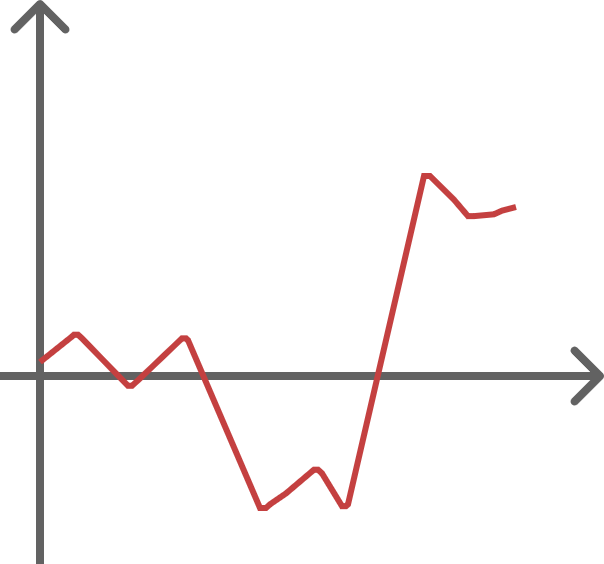
\includegraphics[width=\textwidth]{figures/prelem/timeseries.png}
        \caption{Data Series}
        \label{fig:dataseries}
    \end{subfigure}
    \hfill
    \begin{subfigure}[b]{0.22\textwidth}
        \centering
        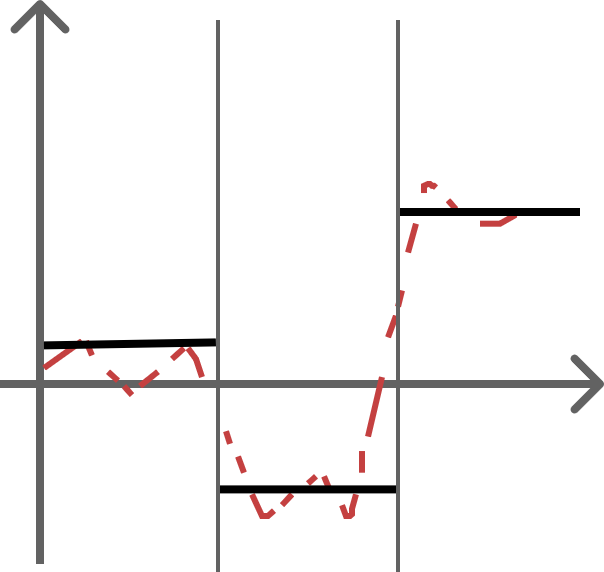
\includegraphics[width=\textwidth]{figures/prelem/PAA.png}
        \caption{PAA Summary}
        \label{fig:PAA}
    \end{subfigure}
    \hfill
    \begin{subfigure}[b]{0.30\textwidth}
        \centering
        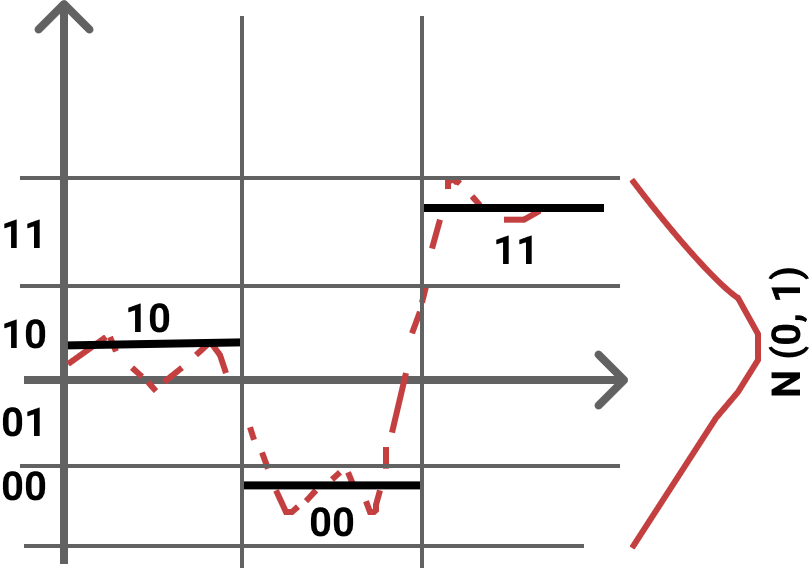
\includegraphics[width=\textwidth]{figures/prelem/isax.png}
        \caption{iSAX Summary}
        \label{fig:iSAXSummary}
    \end{subfigure}
    \hfill
    \begin{subfigure}[b]{0.48\textwidth}
        \centering
        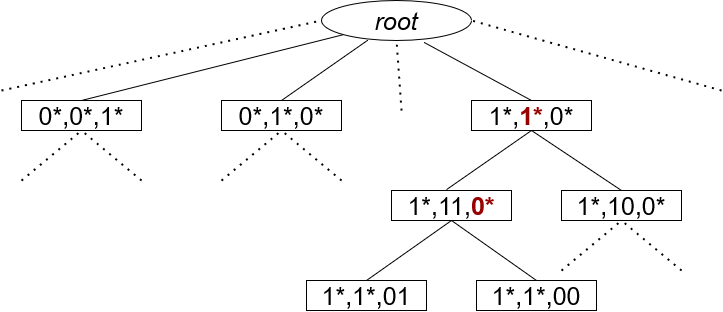
\includegraphics[width=\textwidth]{figures/prelem/isaxTreeCustom.png}
        \caption{iSAX Tree}
        \label{fig:iSAXTree}
    \end{subfigure}
    
    \caption{From data series to iSAX index}
    \label{fig:from_ds_to_iSAX}
\end{figure}

\noindent{\bf Similarity Search}  
We focus on \textit{exact similarity search} (also known as exact \textit{1-NN}),  
which retrieves the data series from a collection that is most similar to a given 
query series. Similarity is typically measured using \textbf{Euclidean Distance (ED)},
but our techniques are general enough to support other widely used 
\textit{similarity measures}, such as Dynamic Time Warping (DTW)~\cite{rakthanmanon2012searching}.  
% 
The \textbf{Euclidean distance} between two time series  
\( T = \{t_1, ... , t_n\} \) and \( T' = \{t'_1, ... , t'_n\} \)  
is defined as:  
\[
ED(T, T') = \sqrt{\sum_{i=1}^{n} (t_i - t'_i)^2}
\]  
% 
We refer to the distance between the \textit{iSAX summaries} of two data series  
as the \textbf{lower-bound distance}.  
The calculation of this distance guarantees the \textbf{pruning property}:  
the lower-bound distance between two data series is always less than or equal to  
their Euclidean distance, which we refer to as the \textbf{real distance}.  
% 
This property enables efficient pruning of candidates during query processing:  
a data series can be \textbf{pruned} if its lower-bound distance to the query series
\( Q \) is greater than the real distance of any other data series in the collection 
from \( Q \).

\noindent
{\bf Leaf-Oriented Trees.}  
In a \textit{leaf-oriented tree}, all data are stored in the leaves, with each leaf
capable of holding up to \( M \) keys.  
% 
During an insertion, if the target leaf \( \ell \) has available space,  
the new key is simply added to \( \ell \).  
However, if \( \ell \) is full, it undergoes a \textbf{split}: it is replaced 
by a subtree consisting of an internal node and two new leaves.  
The keys from \( \ell \) are then redistributed between the new leaves based on
their values.  
% 
If one of the newly created leaves remains empty after redistribution,  
the splitting process is repeated until both leaves contain keys.  

\noindent\textbf{iSAX-Based Indexing.}
Concurrent iSAX-based indexes~\cite{peng2018paris,parisplus,peng2020messi,  
PFP21-I,PFP21-II} operate in two main phases:  
the \textit{tree index construction phase} and the \textit{query answering phase},  
each utilizing distinct data structures. 
During the \textbf{tree index construction phase}, a set of \textit{worker threads}  
processes a collection of input data series (i.e., \textit{raw data}).  
Each series is summarized using an iSAX representation and inserted into a 
\textit{tree index} as a pair of an iSAX summary and a pointer to the corresponding 
data series.  
% 
The process is divided into two main stages:
\begin{itemize}
    \item \textbf{Buffers Creation:} iSAX summary pairs are first stored in array-based  
    \textit{summarization buffers}.  
    \item \textbf{Tree Population:} Worker threads traverse these buffers and insert 
    their entries into the tree index.  
\end{itemize}  
Data series with similar iSAX representations are placed in the same buffer and later  
within the same subtree of the index tree.  
This approach ensures \textbf{high parallelism}, \textbf{good locality}, and  
\textbf{low synchronization overhead} during index construction.

\bigskip  
\noindent\textbf{Query Answering.}  
Given a query data series \( Q \), the system follows these steps:  
\begin{enumerate}
    \item The iSAX summary of \( Q \) is computed and used to traverse the index tree,  
    leading to a leaf \( \ell \).  
    \item The \textit{real distance} between \( Q \) and each data series in \( \ell \) is computed.  
    \item The smallest distance found so far is stored in the \textbf{Best-So-Far (BSF)} variable,  
    serving as an initial approximate answer.  
\end{enumerate}  
Query answering proceeds in two stages:  
\begin{itemize}
    \item \textbf{Pruning Stage:}  
    \begin{itemize}
        \item A set of \textit{query answering threads} traverse the tree.  
        \item If the \textit{lower bound distance} from a node to \( Q \) exceeds BSF,  
        the node is \textit{pruned} and ignored in further processing.  
        \item This guarantees that no pruned data series can be the final answer.  
    \end{itemize}
    \item \textbf{Refinement Stage:}  
    \begin{itemize}
        \item Candidate series are stored in one or more \textit{priority queues}~\cite{parisplus,PFP21-I,PFP21-II}.  
        \item Multiple threads process these candidates, calculating their exact distances to \( Q \).  
        \item BSF is updated whenever a smaller distance is found.  
    \end{itemize}
\end{itemize}   
At the end of this phase, the final answer is contained in BSF.  
\textit{Barriers} synchronize threads at the end of each stage, ensuring correctness,  
while \textit{locks} handle concurrent access to shared data structures.  
Figures~\ref{fig:example} and~\ref{fig:example2} summarize the indexing process.  

\begin{figure}[H]
    \centering
    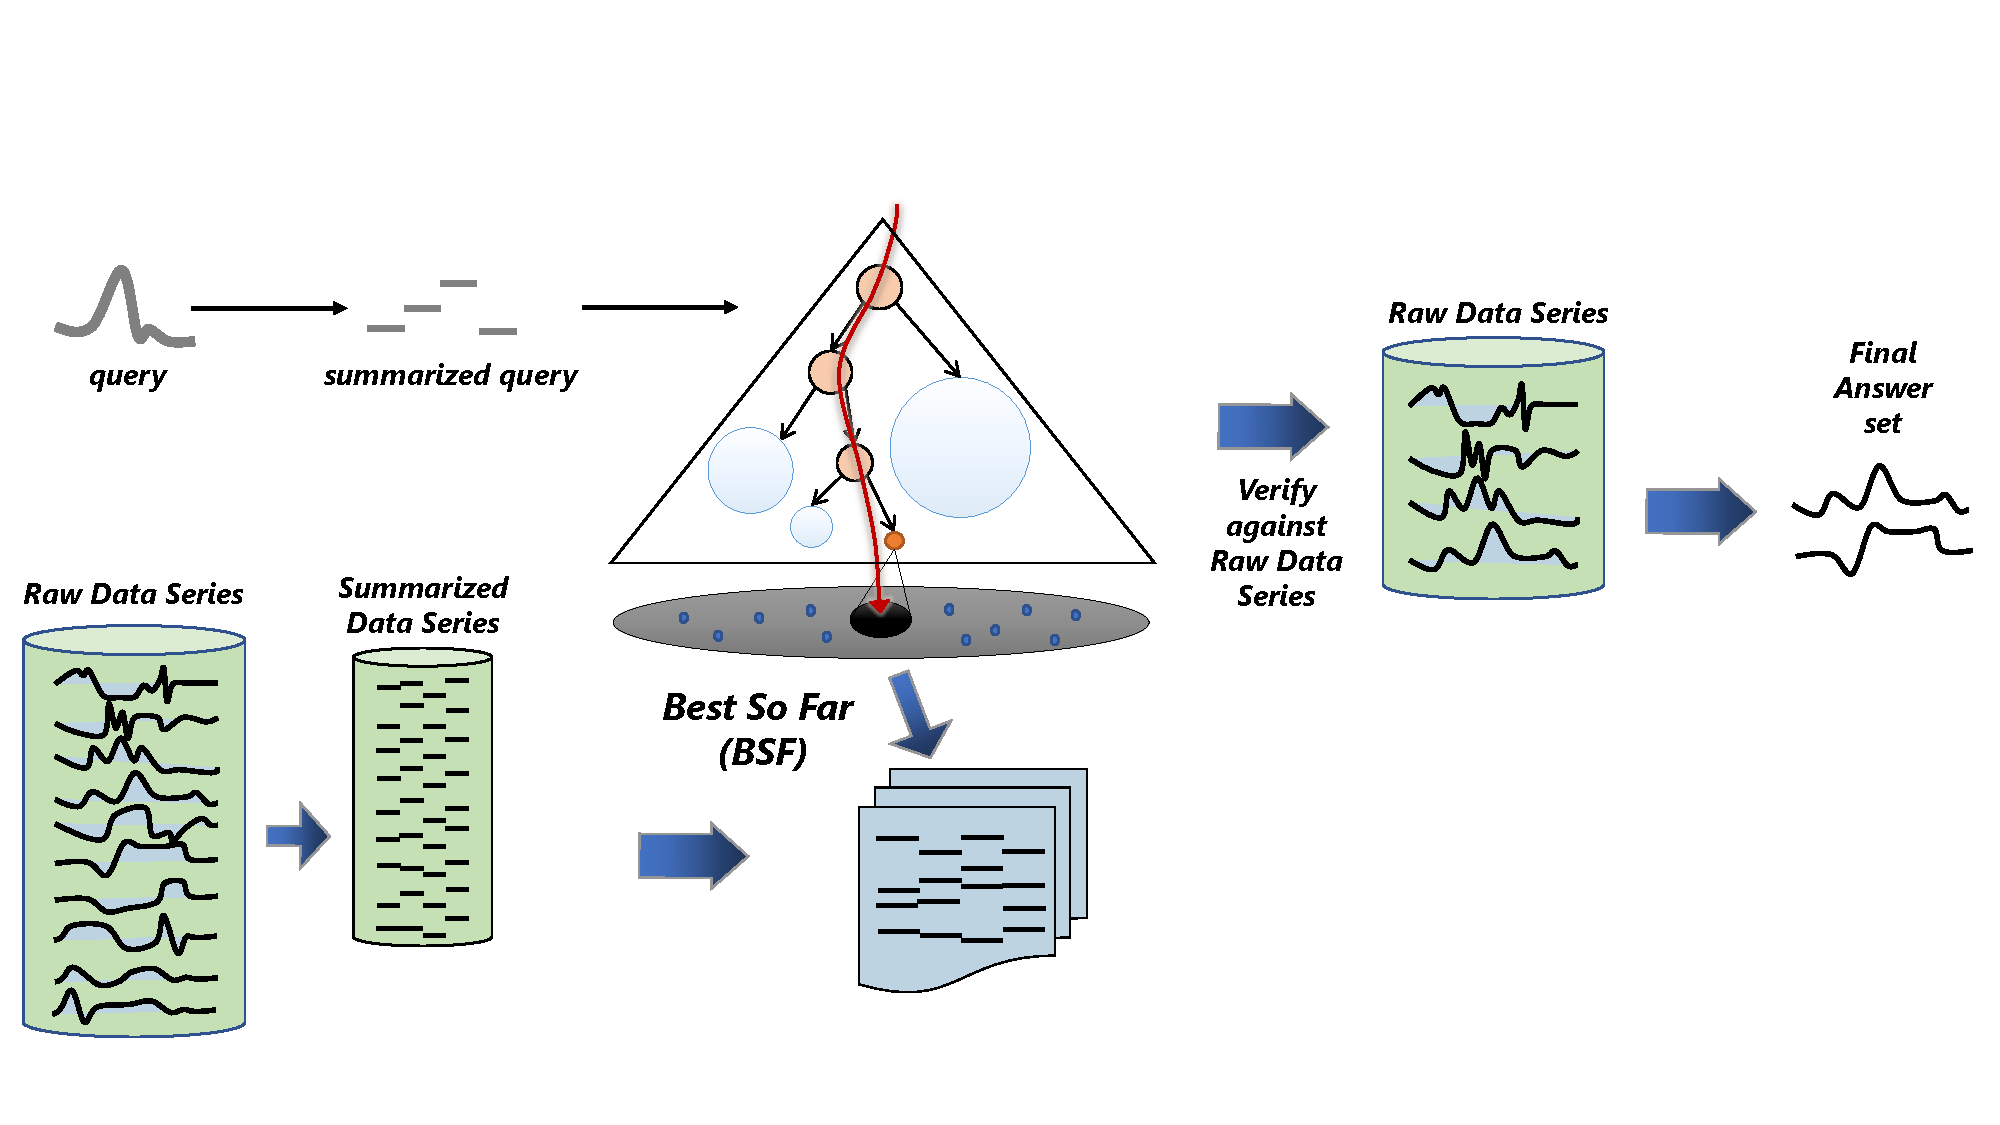
\includegraphics[width=0.5\textwidth]{figures/prelem/iSAX-index.pdf}
    \caption{Similarity search with the use of a data series index.}
    \label{fig:example}
    \vspace{-0.5cm} % Reduces space after the figure
\end{figure}

\begin{figure}[H]
    \centering
    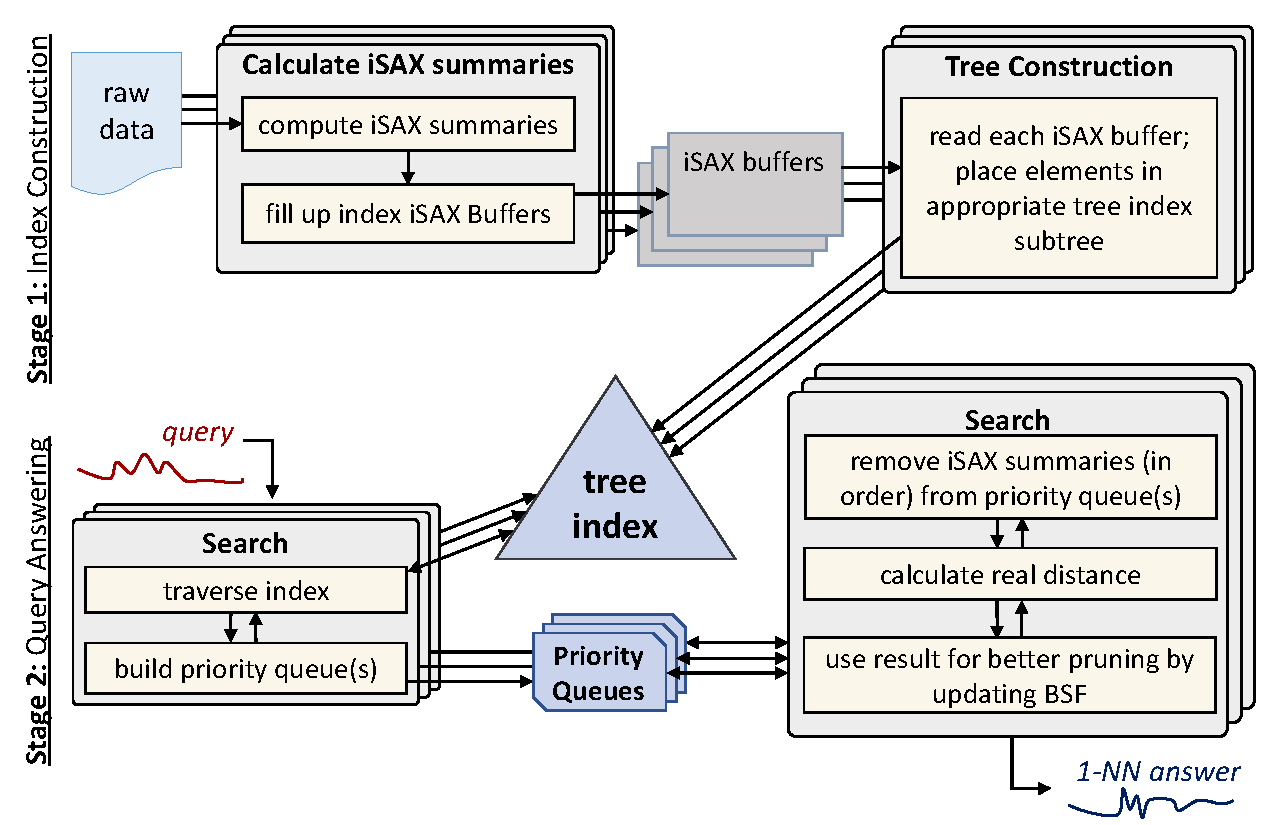
\includegraphics[width=0.5\textwidth]{figures/prelem/flowchart2.pdf}
    \caption{Index building and query answering flowchart for the MESSI data series index.}
    \label{fig:example2}
    \vspace{-0.5cm} % Reduces space after the figure
\end{figure}


\noindent{\bf MESSI as an example.} 
MESSI~\cite{peng2020messi} is a state-of-the-art, in-memory iSAX-based index.
It uses an array, referred to as \textit{RawData}, to store the raw data. During the 
{\em buffers creation stage}, this array is split into a number of fixed-size chunks 
containing consecutive raw data series. Worker threads repeatedly {\em acquire} and
process these chunks, storing the calculated iSAX summaries in the appropriate 
summarization buffers. Threads determine which chunks to work on using a \FAI\ object.
Each thread is allocated its own space in each summary buffer to avoid collisions when
adding elements, ensuring thread safety. This process continues until all data series in
\textit{RawData} have been processed.
% 
During the {\em tree population stage}, worker threads again use \FAI\ to {\em acquire}
iSAX buffers to work on. Each subtree of the index tree is a binary leaf-oriented tree
with fat leaves.
% 
In the {\em query answering phase}, a query answering worker repeatedly {\em acquires}
a subtree (using \FAI) and {\em traverses} it by calculating the {\em lower-bound
distance} between the query series \( Q \) and the iSAX summary of each node
encountered. If the lower-bound distance of a leaf is smaller than the Best So Far (BSF)
distance, the leaf is inserted into a set of {\em priority queues}, with the distance
used as the priority. Threads insert elements into these queues in a round-robin fashion.
Since a priority queue may be concurrently accessed by multiple threads, 
MESSI employs a coarse-grain {\em lock} for synchronization.
% 
During the {\em refinement phase}, each query answering thread \( t \) is assigned a 
priority queue \( \mathit{PQ} \) to process. It repeatedly removes the leaf with the
minimum priority from \( \mathit{PQ} \) and compares its iSAX summary to the BSF.
If the leaf's summary is smaller, the real distances between the data series stored
in the leaf and the query series are computed. Otherwise, the leaf and all remaining
nodes in the queue are pruned. Since multiple threads may process a priority queue
concurrently, it is protected by a coarse-grain lock. Once processing of a priority
queue is complete, thread \( t \) moves on to the next priority queue in a round-robin
manner.
% 
{\em Barriers} are used among threads at the end of each stage and before the start of 
the next to ensure correct synchronization and maintain the integrity of the process.

\noindent{\bf System.}  
We consider a shared-memory system with \( N \) threads that execute {\em concurrently
and asynchronously} while communicating by accessing shared objects. A shared object
\( O \) can be atomically read or written. Additionally, the operation \FAI(O, v)
atomically reads the current value of \( O \), adds the value \( v \) to it, and
returns the value that was read. The operation \CAS($O, u, v$) reads the value of
\( O \), and if it is equal to \( u \), it changes it to \( v \) and returns
\textit{True}; otherwise, \( O \) remains unchanged and \textit{False} is returned.
% 
Threads may experience delays (e.g., due to page faults, power consumption issues,
or overheating~\cite{inteloverheating}), or they may fail by crashing (e.g., due to
software errors). An algorithm is said to be {\em blocking} if a thread must wait for
actions to be performed by other threads in order to make progress. {\em Lock-freedom}
guarantees that the system as a whole continues to make progress, independently of the
speed of threads or their failures.


\subsection{Other Related Work}
Numerous tree-based techniques for efficient and scalable data series similarity search
have been proposed~\cite{DBLP:journals/pvldb/EchihabiZPB18, DBLP:journals/pvldb/EchihabiZPB19,
DBLP:conf/edbt/EchihabiZP21, DBLP:journals/pvldb/EchihabiPZ21},
including approximate~\cite{DBLP:journals/pvldb/AziziEP23, 
DBLP:journals/kais/LevchenkoKYAMPS21} and 
progressive~\cite{DBLP:conf/sigmod/GogolouTEBP20, DBLP:journals/tvcg/JoSF20,
DBLP:conf/sigmod/LiZAH20, DBLP:journals/vldb/EchihabiTGBP23} solutions.
Among these, iSAX-based indexes~\cite{isaxfamily} have proven to be particularly
competitive in terms of both index construction and query performance~\cite{DBLP:journals/pvldb/EchihabiZPB18,
DBLP:journals/pvldb/EchihabiZPB19, hercules, odyssey, dumpy}. These indexes also include
parallel and distributed solutions that leverage modern hardware (e.g., SIMD, multi-core,
multi-socket, GPU), such as ParIS+~\cite{parisplus}, MESSI~\cite{PFP21-I}, and SING~\cite{PFP21-II},
as well as distributed approaches like DPiSAX~\cite{dpisax, dpisaxjournal} and
Odyssey~\cite{odyssey}.
% 
The first lock-free concurrent search tree implementation was proposed in~\cite{EFRB10}.
Building on the ideas from that paper, we develop a baseline algorithm, which we discuss
and compare experimentally with \textit{FreSh} in Section~\ref{section:evaluation}.
Several other non-blocking concurrent search trees have been introduced in the 
literature~\cite{BER14, HL16, ABF20, HJ12, NRM20, CNT14, BP12, EFHR14, FR2018, ABF+22}.
The key novelty of our tree implementation, presented in Section~\ref{sec:fresh}, is its
ability to concurrently perform multiple insert operations in a lock-free manner to
update the array in a (fat) leaf. Additionally, it supports the expeditive-standard mode
of execution. These advancements result in improved parallelism and better performance.
Our approach focuses solely on the functionality required for implementing traversal objects,
whereas the aforementioned implementations support a variety of other features or are designed
for different contexts.
% 
Concurrent priority queues have been explored in~\cite{AK15-I, RT21, WG15, SUNDELL2005609,
tamir_et_al, LJ13}, none of which are based on sorted arrays or support different
execution modes. In our baseline lock-free implementations, we use a skip-list-based
priority queue~\cite{LJ13}, which has been shown to perform well. However, our experiments
indicate that the priority queue design we implemented for \textit{FreSh} significantly
outperforms this approach (Section~\ref{section:evaluation}).
% 
Universal constructions~\cite{FK11spaa, FK12ppopp, FK14, FK17opodis, FK09, FK20,
FKK18, EF+16, FKK22} can provide wait-free or non-blocking concurrent versions of any
sequential data structure. However, due to their general nature, they are often less
efficient than implementations tailored to specific data structures. The algorithms
in~\cite{FK11spaa, FK14, FKK22} are highly efficient for small shared objects
(e.g., stacks and queues) but are not suitable for our application.
% 
The concept of transforming algorithms to achieve different progress guarantees is not
new, as seen in~\cite{SP14, ELM05, GKK06}, though these transformations address different
problems. The technique used in \textit{FreSh}, called \textit{ReFreSh}  departs from all these
prior approaches.

\subsection{Data Streams and Timestamps}
In the context of data streams~\cite{}, timestamps are used to manage sliding windows and to
ensure that data is processed in a meaningful order. Timestamps can either be explicit
or implicit, depending on the source of the data and the importance of time in the data's
semantics. Explicit timestamps are assigned when the exact moment an event occurs is
significant, such as when dealing with events from a sensor or other real-world sources.
These timestamps help maintain the integrity of the data's temporal ordering, although
challenges arise when tuples arrive out of order. While systems can generally expect a
near-increasing order of timestamps, occasional perturbations necessitate buffering
or other techniques to reorder the data effectively.
% 
On the other hand, implicit timestamps are used when the exact time of an event is not
as critical, but it is important to understand whether the data is recent or old.
Implicit timestamps are assigned automatically by the system, offering more flexibility
in managing data, especially when dealing with data from sources that do not naturally
include timestamps.
% 
For systems that need to process composite tuples from multiple streams, such as in the
case of a join operator, assigning timestamps becomes more complex. One approach is the
best-effort method, where timestamps are assigned based on when the tuple is produced,
offering flexibility at the cost of potentially losing deterministic ordering. A stricter
approach assigns timestamps based on the order of streams and query parameters,
ensuring a more deterministic output at the cost of potentially increased latency
due to buffering.
% 
In our system \textit{DFreSh}, we follow the stricter approach to timestamping, ensuring deterministic
ordering and precise synchronization across concurrent updates and queries.
The principles behind this approach are drawn from the work presented 
in \textit{Models and Issues in Data Stream Systems}~\cite{},
which guided the design and implementation of timestamps in our dynamic system.

























% %BIB
\bibliographystyle{plain}
\cleardoublepage
\addcontentsline{toc}{chapter}{Bibliography}
\bibliography{bib/thesis}



\end{document}
